This chapter describes the implementation of the cached profiles functionality for HotSpot, written as part of this thesis.
HotSpot is a vital part of the open source Java Platform implementation, \texttt{OpenJDK}, and the source code is available at \url{http://openjdk.java.net/}.
\\\\
Most of the code additions are included in two new classes \texttt{/share/vm/ci/ciCacheProfiles.cpp} and \texttt{/share/vm/ci/ciCacheProfilesBroker.cpp} as well as significant changes to \\\texttt{/share/vm/ci/ciEnv.cpp} and \texttt{/share/vm/compiler/compileBroker.cpp}.
\\
The core functionality is located in \texttt{/share/vm/ci/ciCacheProfiles.cpp}, a class that takes care of setting up the cached profile data structure as well as providing public methods to check if a method is cached or not. The class \texttt{/share/vm/ci/ciCacheProfilesBroker.cpp} is used before a cached method is compiled. It is responsible for setting up the compilation environment, so the JIT compiler can use the cached profiles.
\\\\
A full list of modified files and the changes can be seen in the webrev at \url{http://mohlerm.ch/b/webrev.01/} or Appendix \ref{a:codechanges}.
The changes are provided in form of a patch for HotSpot version 1aef080fd28d. In the following, the original version is referred to as \textit{baseline}.
\\\\
We will describe and explain the functionality and the design decisions in the following sections, ordered by their execution order.

\section{Creating cached profiles}
\label{s:creatingprofiles}
The baseline version of HotSpot already offers a functionality to replay a compilation based on previously saved profiling information.
This is mainly used in case the JVM crashes during a JIT compilation to replay the compilation process and allow the JVM developer to further investigate the cause of this incident.
Apart from this automatic process, there exists the possibility to invoke the profile saving manually by specifying the \texttt{DumpReplay} compile command option per method.
\\\\
We introduce a new method option called \texttt{DumpProfile} as well as a new compiler flag \newline\texttt{-XX:+DumpProfiles} that appends profiling information to a file as soon as a method gets compiled. The first option can be specified as part of the \texttt{-XX:CompileCommand} or \texttt{-XX:CompileCommandFile} flag and allows the user to select single methods to dump their profile. The second command dumps profiles of all compiled methods.
The profile is converted to a string and saved in a simple text file called \textit{cached\_profiles.dat}.
\\\\
The system will only consider compilations of Level 3 or Level 4. Level 1 and Level 2 are rarely used in practice and do only include none or little profiling information. The user can also restrict the profiles to Level 4 by using the compiler flag: \texttt{-XX:DumpProfilesMinTier=4}.
\\\\
The dumped profiling information consists of multiple \texttt{ciMethod} entries, \texttt{ciMethodData} entries, and one \texttt{compile} entry. They are separated by line breaks and keywords to make sure the data can be parsed easily. A shortened example of a cached profile can be found in Appendix \ref{a:cacheprofileexample}. The \texttt{ciMethod} entries contain information about the methods used in the compilation (Table \ref{t:cimethod} describes it in more detail). The \texttt{ciMethodData} (see Table \ref{t:cimethoddata}) includes all profiling data about the methods itself to be able to redo the compilation.
The compile entry saves the bytecode index in case of OSR, the level of the compilation and lists all inlining decisions (Table \ref{t:compile}).
\\\\
A method can be compiled multiple times and at different tiers, thus compilation information for the same method can be dumped multiple times. This is intentional and is taken care of when loading the profiles (see Section \ref{s:initializingprofiles}).
\begin{table}[ht!]
  \caption{content of ciMethod entry in cached profile}
  \label{t:cimethod}
  \begin{center}
    \begin{tabular}{|p{5cm}|p{10.5cm}|} 
      \hline
       \textbf{name} & \textbf{description} \\ \hline\hline
       class\_name,& used to identify the method\\
       method\_name, & \\
       signature & \\ \hline
       invocation\_counter & number of invocations\\ \hline
       backedge\_counter & number of counted backedges\\ \hline
       interpreter\_invocation\_count & number of invocations during interpreter phase\\ \hline
       interpreter\_throwout\_count & how many times method was exited via exception while interpreting\\ \hline
       instructions\_size\_name & rough size of method before inlining\\ \hline
    \end{tabular}
  \end{center}
\end{table}
\begin{table}[ht!]
  \caption{content of ciMethodData entry in cached profile}
  \label{t:cimethoddata}
  \begin{center}
    \begin{tabular}{|p{5cm}|p{10.5cm}|} 
      \hline
       \textbf{name} & \textbf{description} \\ \hline\hline
       class\_name,& used to identify the method\\
       method\_name, & \\
       signature & \\ \hline
       state & if data is attached and matured\\ \hline
       current\_mileage & maturity of the oop when snapshot is taken\\ \hline
       orig &  snapshot of the original header\\ \hline
       data & the actual profiling data\\ \hline
       oops & ordinary object pointers, JVM managed pointers to object\\ \hline        
    \end{tabular}
  \end{center}
\end{table}
\begin{table}[ht!]
  \caption{content of compile entry in cached profile}
  \label{t:compile}
  \begin{center}
    \begin{tabular}{|p{5cm}|p{10.5cm}|} 
      \hline
       \textbf{name} & \textbf{description} \\ \hline\hline
       class\_name,& used to identify the method\\
       method\_name, & \\
       signature &\\ \hline
       entry\_bci & byte code index of method\\ \hline
       comp\_level & compilation level of record\\ \hline
       inline & array of inlining information\\ \hline        
    \end{tabular}
  \end{center}
\end{table} 
\section{Initializing cached profiles}
\label{s:initializingprofiles}
The information dumped in step \ref{s:creatingprofiles} can now be used in a next run of that particular program.
To specify that profiles are available, we introduce a new compiler flag \texttt{-XX:+CacheProfiles} that enables the use of previously generated profiles. By default, it reads from a file called \textit{cached\_profiles.dat} but a different file can be specified using:\\ \texttt{-XX:CacheProfilesFile=other\_file.dat}.
\\\\
Before any cached profiles can be used the virtual machine has to parse that file and organize the profiles and compile information in a data structure. This data structure is completely kept in memory during the whole execution of the JVM to avoid multiple disk accesses.
The parsing process is invoked during boot up of the JVM, directly after the compileBroker gets initialized. This happens before any methods are executed and blocks the main thread of the JVM until finished.
\\\\
As mentioned in Section \ref{s:creatingprofiles}, the file consists of method information, method profiles, and additional compile information. The parser scans the file once and creates a so called \texttt{CompileRecord} for each of the methods that includes compilation information in the file. This compile record also includes the list of method information (\texttt{ciMethod}) and their profiling information (\texttt{ciMethodData}).
As mentioned previously, a method's compile information could have been dumped multiple times, which results in multiple \texttt{CompileRecords} for the same method. In this case, HotSpot will only keep the \texttt{CompileRecords} based on the latest data written to the file but never overwrite an existing higher level profile.
Because a profile dumped by the C1 compiler can not be used by the C2 compiler and the other way around, the level of the profile matters as it influences the compile level transitions described in Section \ref{s:cacheprofilesmode}.
And since profiling information only grows, the compilation that happened last contains the richest profile and is considered the best.
This is based on the fact that the richer the profile, the more information about the method execution is known and influences the compiled version of that method. For example, a profile for a method might include data for all its branches and can therefore help avoid running into uncommon traps and trigger deoptimizations.
Unfortunately, the last profile might not necessarily be the best to use. It can happen, that a cached profile includes classes that are not yet loaded and therefore some optimizations are not possible. In this case an earlier profile could be better.
\\\\
The \texttt{CompileRecord} as well as the lists of method information and profiles are implemented as an array located in HotSpot's heap space.
They get initialized with a length of 8 and grow when needed. This choice has been done for simplicity and leaves room for further improvements.

\section{Using cached profiles}
\label{s:usingprofiles}
The implementation offers three different modes: \texttt{Mode 0}, \texttt{Mode 1}, and \texttt{Mode 2}, that differ in the way they use the cached profiles.
The following paragraph applies to all three modes and we will discuss the differences of the modes in detail in Section \ref{s:cacheprofilesmode}.
\\\\
The idea is to modify the compiler to use cached profiles if available and continue as usual otherwise.
A simplified graphical overview of the program flow for compiling a method with the changes introduced in this thesis can be found in Figure \ref{f:programflow}.
\begin{figure}[ht!]
  \begin{center}
    \centering
    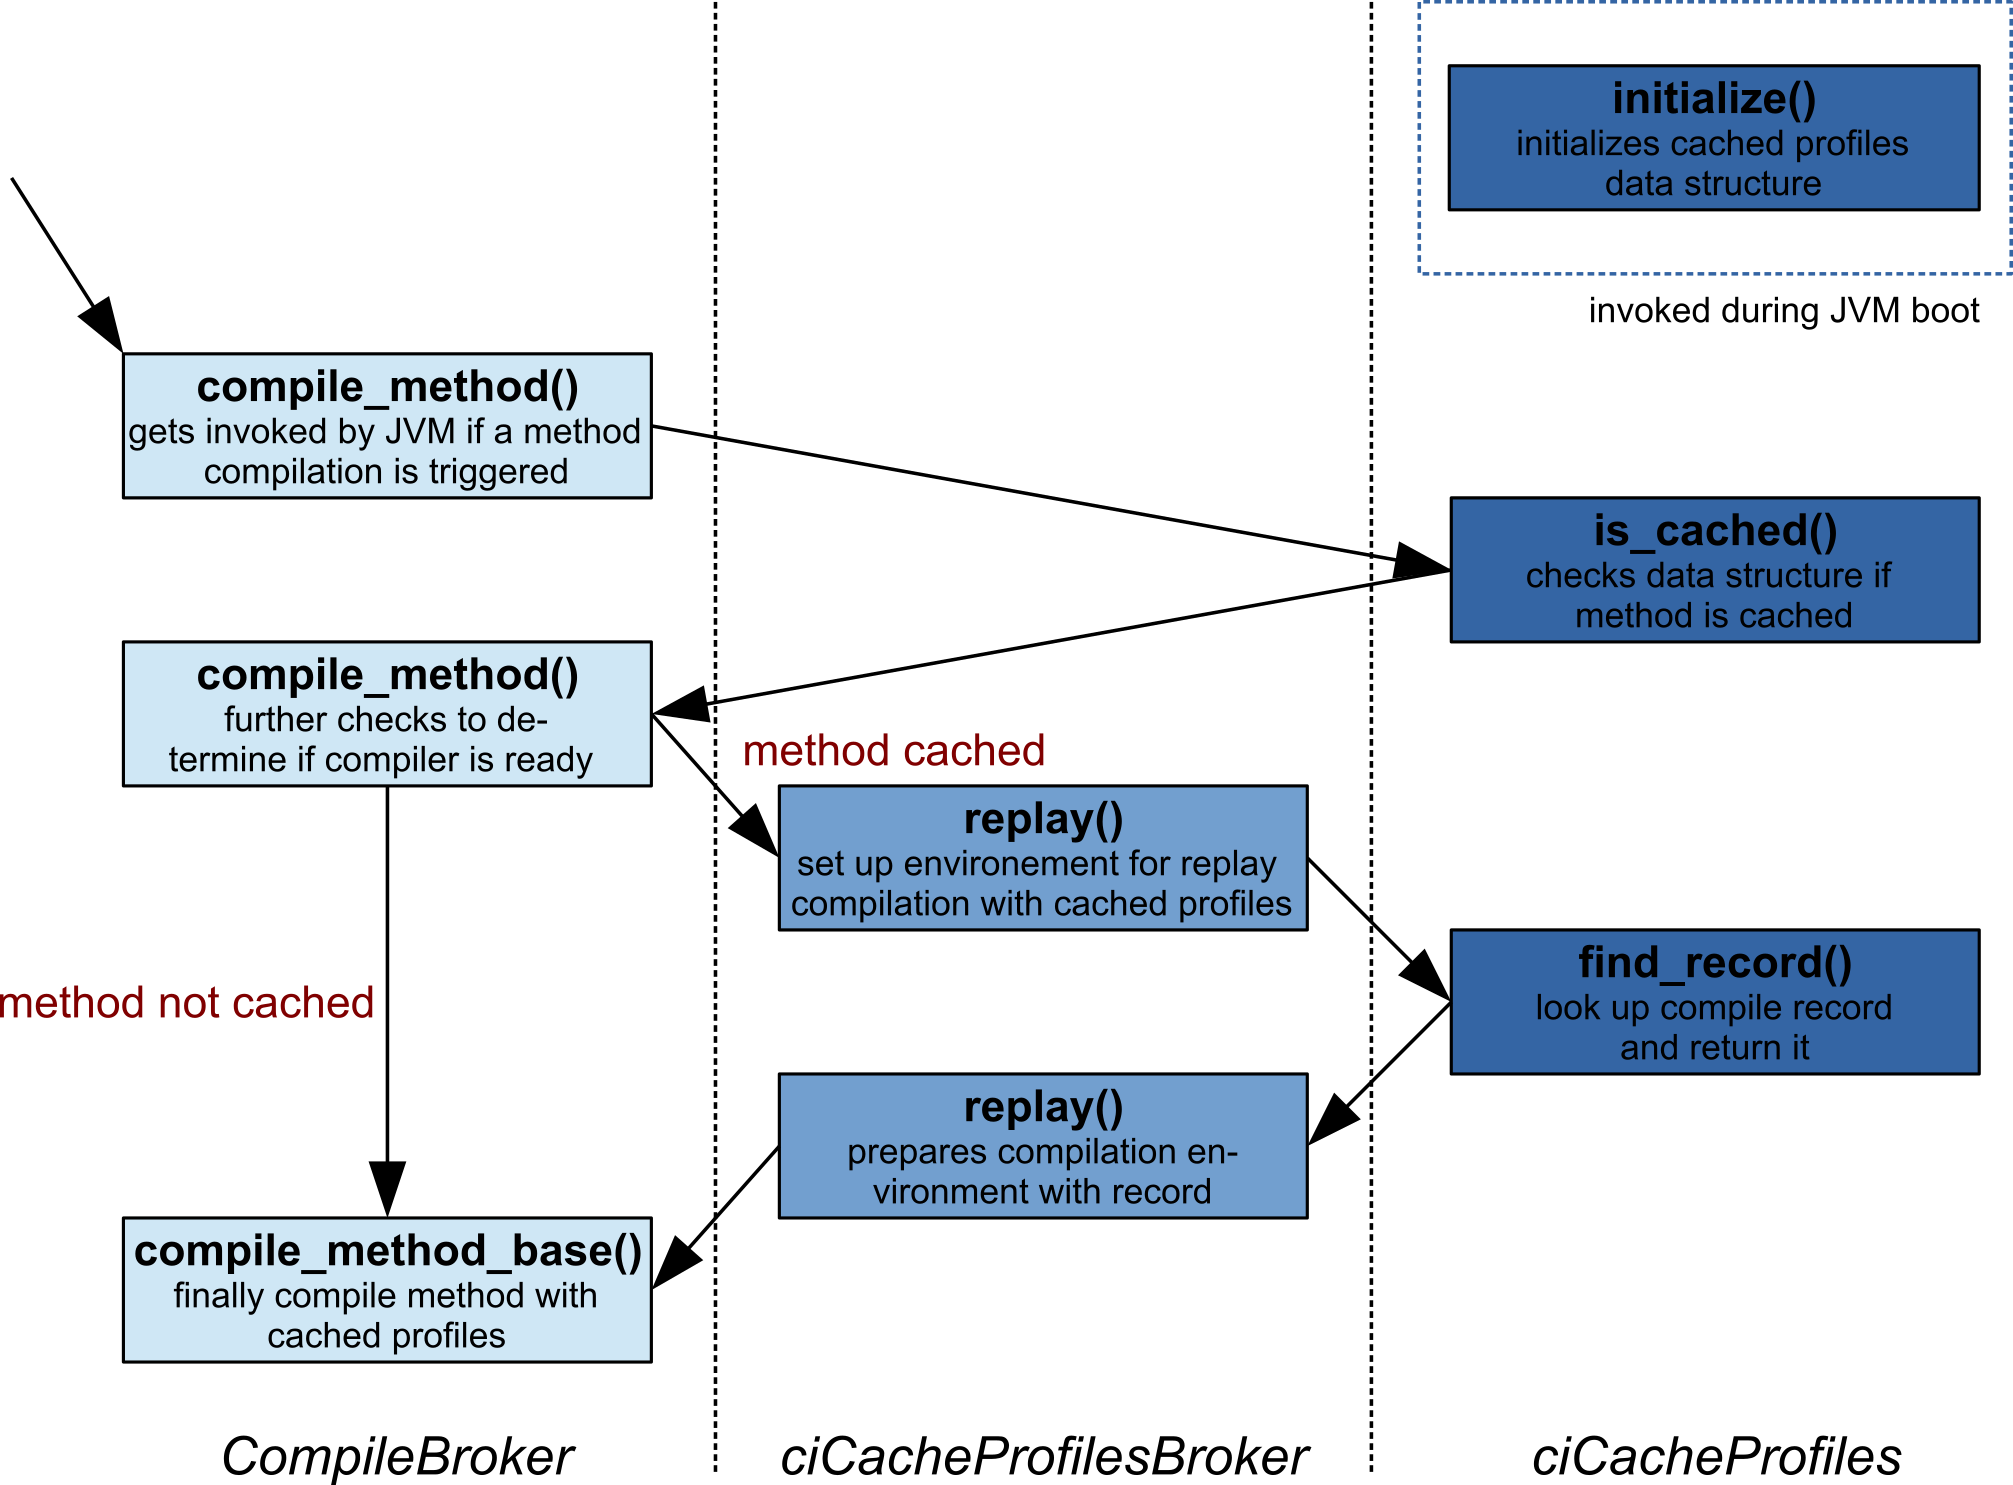
\includegraphics[width=0.8\textwidth]{figures/program_flow.png}
    \caption{program flow for compiling a method}
    \label{f:programflow}
  \end{center}
\end{figure}\\
As mentioned before, once compilation thresholds are exceeded a method is scheduled for compilation. This means that the JVM will invoke a method called \texttt{compile\_method()}, located in the \texttt{compileBroker} class. This method tests if certain conditions hold, for example, it checks if the compile queue is not full or if there is already another compilation of that particular method running.
We extended this method with a call to \texttt{ciCacheProfiles::is\_cached(Method* method)} which does a linear scan through the \texttt{CompileRecord} array data structure. The method returns either 0 if the method is not cached or returns an integer value, reflecting the compile level, in case a cached profile of this method is available. Because only methods compiled with level 3 or 4 are cached, this call to \texttt{is\_cached()} only gets executed if the compilation request is also of level 3 or higher.\\\\
Depending on the compilation level of the profile, the level of the requested compilation, and the \texttt{CacheProfileMode}, the \texttt{compileBroker} then schedules either a compilation using freshly gathered profiles or calls into \texttt{ciCacheProfilesBroker} to replay the compilation, based on a cached profile. In contrast to cached profiles, fresh profiles describe profiles gathered during the current run of the JVM. Since these decisions are different in each mode, a detailed description is provided in the next section.
In case the method is not cached, the execution continues like in the baseline version.
Otherwise, the \texttt{ciCacheProfilesBroker} class then initializes the replay environment and retrieves the compile record from \texttt{ciCacheProfiles}. Subsequently, the needed cached profiles get loaded to make sure they are used by the following compilation. \texttt{ciCacheProfilesBroker} then returns the execution to the \texttt{compileBroker}, which continues with the steps needed to compile the method. Again some constraints are checked (e.g. if there is another compilation of the same method finished in the meantime) and a new compile job is added to the compile queue. Eventually the method is compiled using the cached profiles.
\\\\
Since the implementation is only invoked by the static class \texttt{compileBroker}, \texttt{ciCacheProfiles} and \texttt{ciCacheProfilesBroker} are static classes as well. The \texttt{compileBroker} is solely called by the JVM main thread, therefore there is no need to make the compileRecord data structure or any of the new methods thread safe. 

\section{Different usage modes for cached profiles}
\label{s:cacheprofilesmode}
The implementation of cached profiles offers 3 different modes, which differ from each other in the transitions between the compilation tiers.
The motivation as well as the advantages and disadvantages of the modes are described in the following three subsections.
While \texttt{Mode 0} and \texttt{Mode 1} are similar except for the compile thresholds, \texttt{mode2} differs significantly.
Figure \ref{f:hs_tiers_thresholds} provides a graphical overview of the differences in the compilation tier transitions of the modes.
\begin{figure}[h]
  \begin{center}
    \centering
    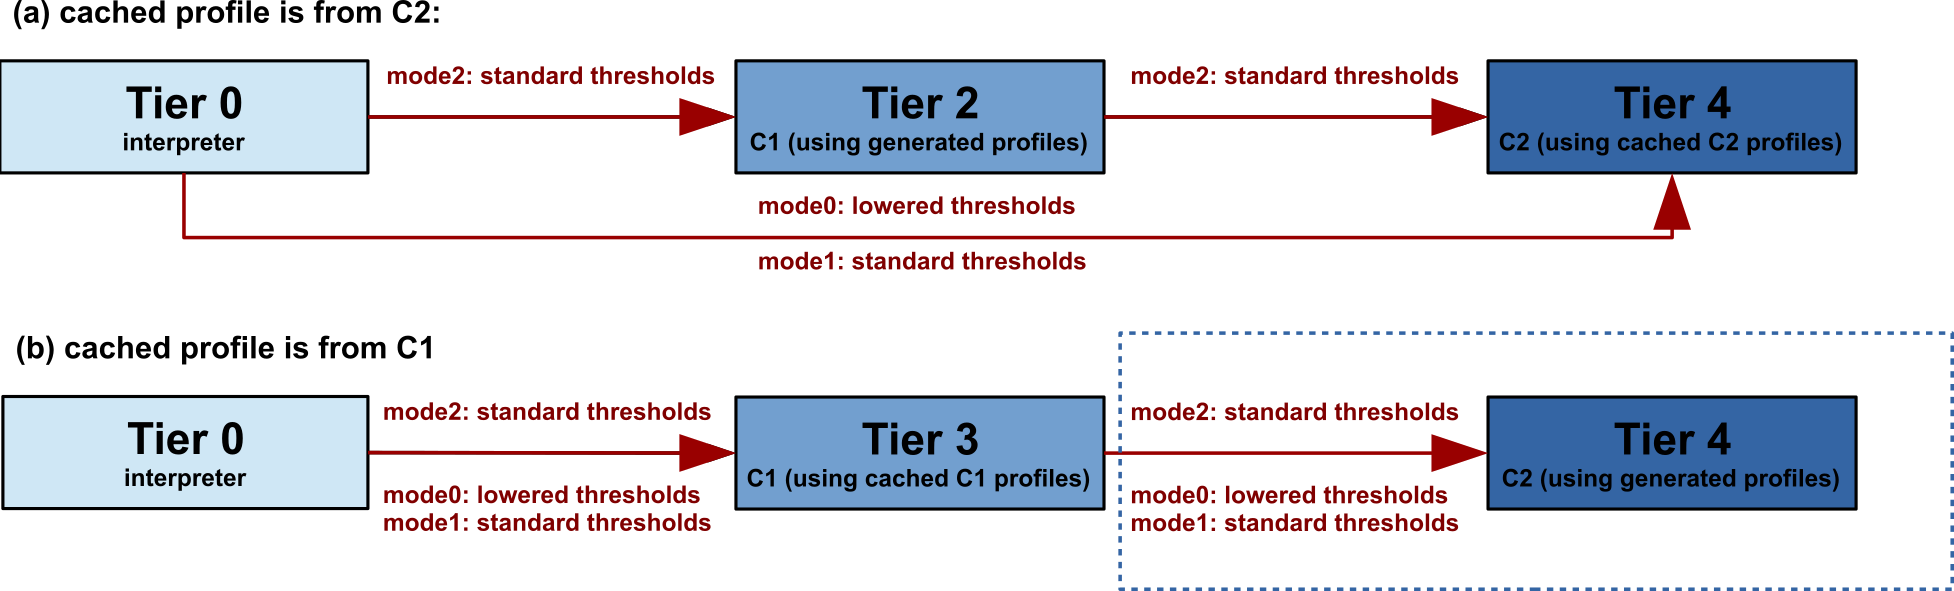
\includegraphics{figures/hs_tiers_threshold.png}
    \caption{Tier transitions of different modes}
    \label{f:hs_tiers_thresholds}
  \end{center}
\end{figure}\\
All three modes have advantages and disadvantages and their performance is evaluated in Chapter \ref{c:performance}. Since depending on the methods, different modes might perform best. It is up to the JVM user to decide which mode he or she wants to use. Because \texttt{Mode 2} is the most conservative one, which does not modify thresholds it is considered the default mode and used if not further specified.

\subsection{Compile thresholds lowered (Mode 0)}
\label{s:mode0}
The first mode is based on the consideration that a method that has a profile available does not require profiling anymore. Therefore, the compile thresholds (see Section \ref{s:compilethresholds}) of these methods are lowered. If the cached method has a C2 profile, all thresholds are lowered, in case of a C1 profile, only the thresholds that affect the tiers below and equal to Tier 3. This differentiation is done to prevent an increase in early C2 compilations using fresh profiles. Because a lower Tier 4 threshold would mean, that a method which only got compiled at Tier 3 when creating the profile, might now trigger a Tier 4 compilation very early. At this point, the fresh profiles generated by the Tier 3 compiled version are still immature. Using them to compile with Tier 4 results in code that includes only limited profiling information, which causes costly deoptimizations when used. 
\\\\
By default, the thresholds are lowered to 1\% of their original values but the threshold scaling can be modified with the JVM parameter: \texttt{-XX:CacheProfilesMode0ThresholdScaling=x.xx}. 1\% results in the Level 3 invocation counter being reduced from 200 to 2. This means that the method will be interpreted once but then trigger a compilation on the next invocation.
Since the interpreter also handles class loading, this decision has been made to avoid the need of loading classes in C1 or C2 which was considered out of the scope for this thesis. HotSpot expects classes of standard libraries to be loaded in a very specific order. Moving class loading to C1 or C2 would mess with that order and can therefore not be done without huge changes to the JVM.
\\\\
In \texttt{Mode 0}, the JIT compiler will always use a cached profile for compilations of Level 3 or Level 4 in case there is a cached profile which has been generated by a compiler of the same level. However, if a method to be compiled on Level 3 has a cached profile available for Level 4, the compiler will skip the C1 compilation and immediately compile with C2. In this case, HotSpot directly uses the highly optimized version generated by C2 and in an ideal case the method will need less time to reach peak performance.
\\\\
However, since the thresholds of all methods with cached profiles get lowered and some of the C1 compilations are promoted to C2 compilations, the C2 compiler is put under heavy load. Especially during startup of a program, where many compilations happen naturally, C2 might not be able to handle all these requests at the same time and the compile queue fills up. This might negatively affect performance and is analyzed in Section \ref{s:perf_compilequeue}.

\subsection{Unmodified compile thresholds (Mode 1)}
\label{s:mode1}
\texttt{Mode 1} is doing exactly the same as \texttt{Mode 0} but does not lower the compilation thresholds of methods with cached profiles.
This is done to reduce the load on C2 as mentioned in Subsection \ref{s:mode0}.
Apart from this change \texttt{Mode 1} has the same behaviour as \texttt{Mode 0}.
\subsection{Modified C1 stage (Mode 2)}
\label{s:mode2}
Both modes mentioned above use cached profiles as soon as a compilation of Level 3 or 4 are triggered. Since the thresholds for Level 3 are smaller than the Level 4 thresholds (see Appendix \ref{a:compilethresholds}) a method reaching a Level 3 threshold could actually trigger a Level 4 compilation, if the cached profile is one of Level 4. So even if \texttt{Mode 1} is used and the thresholds are untouched, C2 might get overloaded since compilations occur earlier.
\\\\
\texttt{Mode 2} has been designed to make as little changes as possible to the tiered compilation and prevent C2 being used more than usual. It does so by keeping the original tiered compilation steps and compilation thresholds and compiles methods with C1 prior to C2. But since there are already profiles available, there is no need to run at Tier 3 to generate full profiles but instead it uses Tier 2.
Tier 2 does the same optimizations but offers only limited profiles like method invocation and backbranch counters. They are needed to know when to trigger the C2 compilation and therefore Tier 1 can not be used. 
By avoiding Tier 3 and using Tier 2 instead methods spend less time in code gathering profiling information and therefore method execution is considered about 30\% faster \cite{code_atp_hpp}.
Eventually, if the Tier 4 thresholds are reached, the method is compiled using C2 and the cached profiles. This still maintains the benefit from having more complete profiles available early but avoids modifying thresholds which could result in a very different load to the compiler. 
\\\\
The above only makes sense if the cached profile is a C2 profile.
If only a C1 profile is available, C1 should gather fresh, full profiles since they might be needed in C2 later. HotSpot will then only use the cached profile during the C1 compilation and then use the generated profiles for possible C2 compilations.
In theory this transition is considered rare, because if a method has not been compiled with C2 when creating the profile it is unlikely to get compiled with C2 in the future.
\\\\
To summarize, we expect a performance benefit C1 compiled code by using Level 2 instead of Level 3 and a benefit for C2 compiled code by using more comprehensive profiles.

\section{Problems}
\label{s:problems}
If the profiles generated by multiple runs of the program deviate sharply it is likely that a cached profile does not fit to the current execution. In this case the compiled version would still trigger many deoptimizations and the method could end up having even worse performance since it's going to use the profile over and over again.
For each method, the JVM maintains a deoptimization counter. Cache profiles are used if the counter is below a certain limit. If they are above that limit a standard compilation using freshly gathered profiles will be used instead.
The limit is 10 to allow a small number of recompilations. This could for example be useful when the method is deoptimized due to classes not being loaded. The value of 10 seems reasonable for all executed measurements.
\section{Debug output}
\label{s:debugoutput}
For debugging and benchmarking purposes four debug flags are implemented, that can be used along with \texttt{-XX:+CacheProfiles}.
\begin{table}[ht]
  \centering
 % \caption{}
  \label{t:debugflags}
  \begin{center}
    \begin{tabular}{| l | p{9.0cm} |}
       \hline
       \textbf{flag} & \textbf{description} \\ \hline\hline
       -XX:+PrintCacheProfiles & enable command line debug output for cached profiles\\ \hline
       -XX:+PrintDeoptimizationCount & prints amount of deoptimizations when the JVM gets shut down\\ \hline
       -XX:+PrintDeoptimizationCountVerbose & prints total the amount of deoptimizations on each deoptimization\\ \hline
       -XX:+PrintCompileQueueSize & prints the total amount of methods in the compile queue each time a method gets added \\ \hline
    \end{tabular}
  \end{center}
\end{table}

 
